\chapter{Impact Study}\label{ch:impacts}

\section{Introduction}

\section{Related Work}

\subsection{Impacts on Cars}

Simulations, Real-World Impacts

\subsection{Impacts on Cyclists}

Simulations, Real-World Impacts

\section{Concept}

\subsection{Final Application Architecture and Design}

\begin{figure}[htbp]
\caption{Final application infrastructure.}\label{fig:architecture}
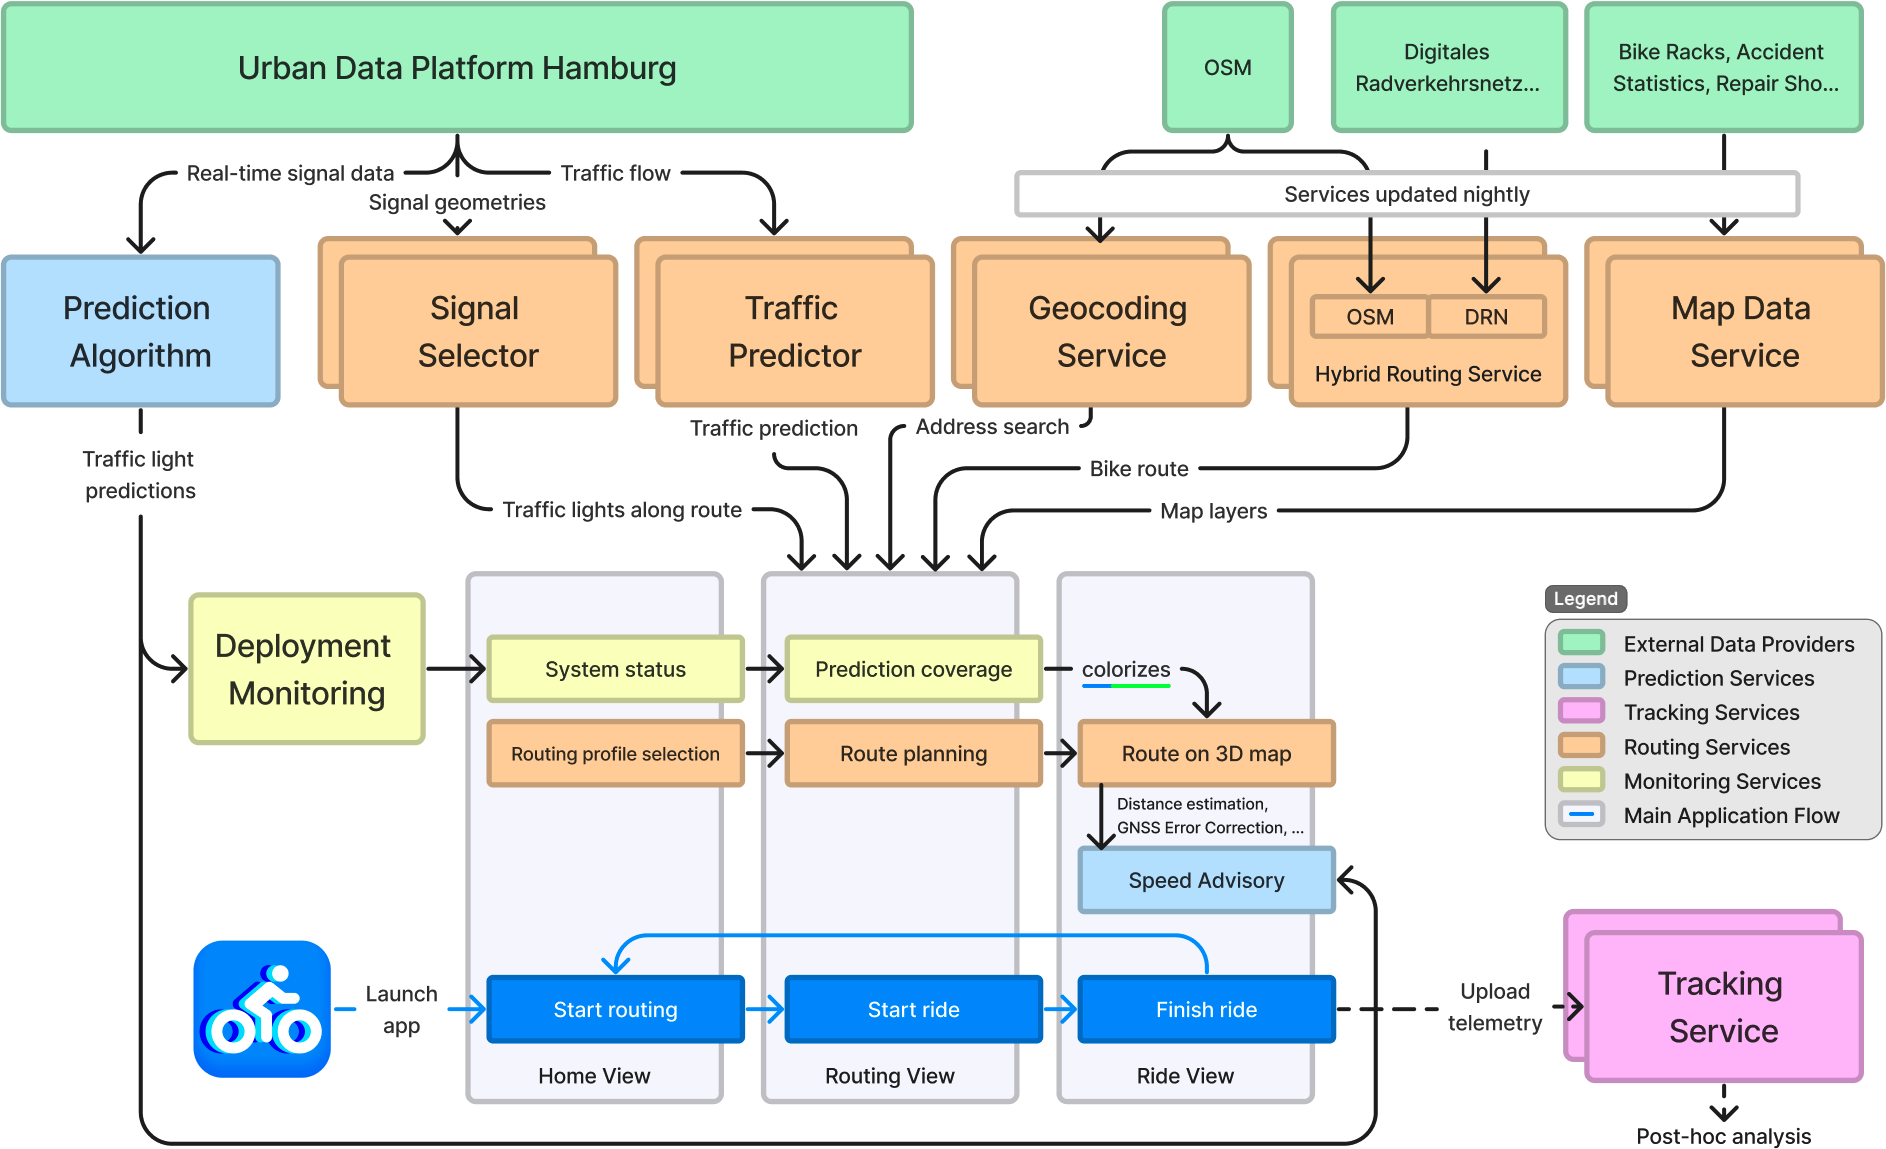
\includegraphics[width=\linewidth]{images/architecture.png}
\end{figure}

\Cref{fig:architecture} highlights the final service infrastructure that combines the developed solutions. The first key solution to make a bike-GLOSA app practical in a real-world urban environment is handling massive amounts of traffic light data. A prediction infrastructure (blue) is proposed that maximizes data ingress stability and self-monitors prediction qualities and availability. These metrics are used within the mobile application to adapt the speed advisory user interface and inform users about data outages.

A speed advisory user interface (the Ride View) is designed that utilizes the speedometer projection to give users a free choice of the desired speed. Uncertainties in the prediction are visualized to enhance the speed advisory's trustworthiness. To make the speed advisory practical, a user-defined route is used for distance-to-signal estimation, traffic light matching, battery-efficient GNSS error correction, and a camera controller for improved traffic light visibility. Combining the speed advisory system with a navigation solution is another key idea to enable these methods and make the mobile application useful in the absence of traffic light predictions.

To deliver bike navigation, a routing infrastructure (orange) is implemented that provides personalized, accurate, and metadata-enhanced bike routing. Once waypoints are found using the Geocoding Service and the Map Data Service that delivers bike-specific points of interest, an accurate bike route is calculated through the developed DRN approach. Route metadata and the predicted traffic situation are visualized to allow for a more informed routing decision. Generated routes are marked green at spots where users can expect a speed advisory. The routing material's actuality is ensured through an automated update CI/CD pipeline. 

The final key solution that connects the speed advisory to the routing is route-based traffic light matching. Multiple approaches were tested, coming to a final machine-learning-based method that compares geometric features between the traffic light geometries and the route geometry to decide which sequence of signals will be passed along the trajectory. To avoid giving a speed advisory for the wrong intersection, unconnected intersections are detected and also matched along the route.

Finally, a tracking service is implemented that obtains ride statistics from users. The collected telemetry data is used to conduct post-hoc analyses on the actual impact of bike-GLOSA on ride behavior. \Cref{ch:results} will focus on the analysis of this data.

\begin{figure}[htbp]
\caption{The PrioBike app's main view flow.}\label{fig:app}
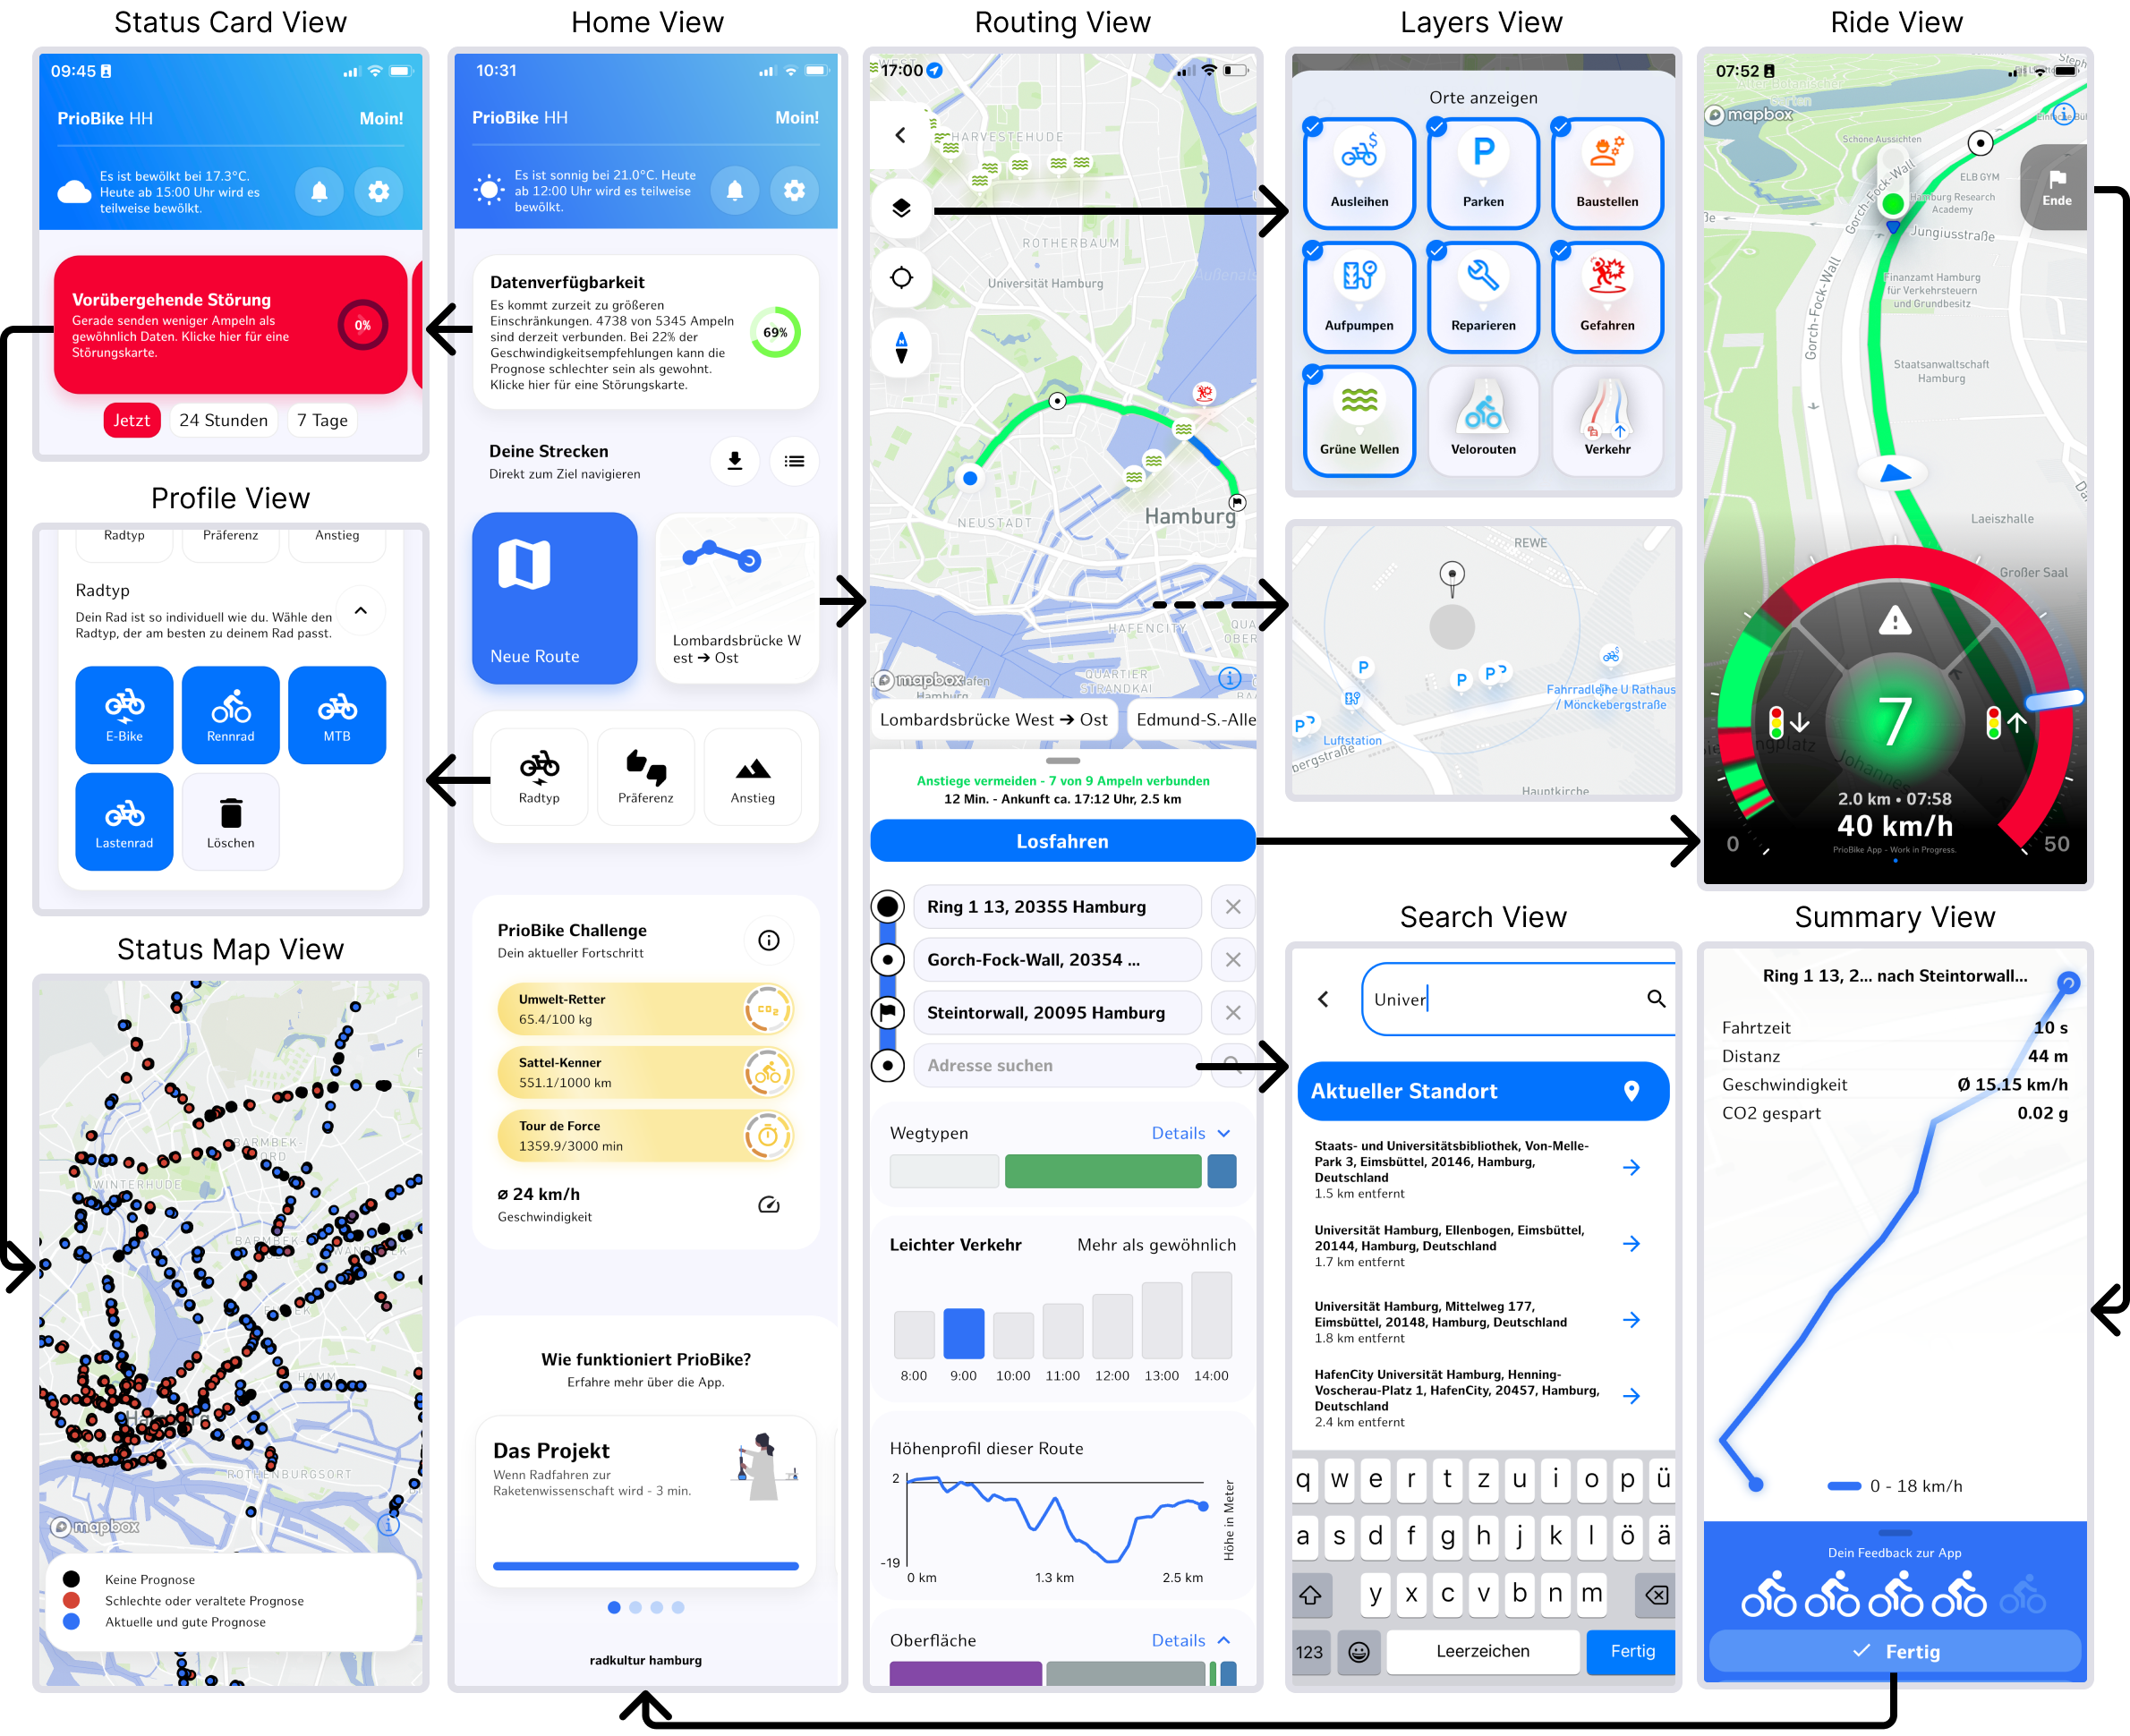
\includegraphics[width=\linewidth]{images/app.png}
\end{figure}

What's visible to the user is an application similar to other navigation apps like Google Maps or Komoot, with added speed advisory functionality. \Cref{fig:app} shows how the designed user interface components are combined into a cohesive application flow concept. From the Home view, which allows users to inform themselves about the current prediction status, users can personalize their routing profile and open the Routing view. This view provides the described route planning functionality. Finally, users can start a ride to obtain the discussed speed advisory. A summary is given after the ride, together with the option to rate the application experience. This rating, together with the collected ride and prediction data, is sent to the tracking service in an optionally offloaded upload routine.

The final application is distributed to real-world test users in Hamburg, who can freely use the app throughout the city to provide realistic experimental circumstances for the urban cycling setting. Based on the collected data, surveys, and other experiments, the next goal is to determine the impacts of such a solution. These aspects will be discussed in the following chapter.

\subsection{User Questionnaire}

\subsection{Collection of Telemetry Data}

\subsection{Detection of Stops at Intersections}

\section{Results}

\subsection{General User Feedback}

\subsection{Reaction to the Speed Advisory}

\subsection{Impact on Stops at Red Lights}

\section{Conclusions}
